\documentclass[american,]{article}
\usepackage{lmodern}
\usepackage{amssymb,amsmath,amsthm}
\usepackage{ifxetex,ifluatex}
\usepackage{fixltx2e} % provides \textsubscript
\ifnum 0\ifxetex 1\fi\ifluatex 1\fi=0 % if pdftex
  \usepackage[T1]{fontenc}
  \usepackage[utf8]{inputenc}
\else % if luatex or xelatex
  \ifxetex
    \usepackage{mathspec}
  \else
    \usepackage{fontspec}
  \fi
  \defaultfontfeatures{Ligatures=TeX,Scale=MatchLowercase}
\fi
% use upquote if available, for straight quotes in verbatim environments
\IfFileExists{upquote.sty}{\usepackage{upquote}}{}
% use microtype if available
\IfFileExists{microtype.sty}{%
\usepackage{microtype}
\UseMicrotypeSet[protrusion]{basicmath} % disable protrusion for tt fonts
}{}
\usepackage[margin=1in]{geometry}
\usepackage{hyperref}
\hypersetup{unicode=true,
            pdftitle={The reference model approach in feature selection problems},
            pdfauthor={Federico Pavone, Juho Piironen, Paul-Christian B\"{u}rkner, Aki Vehtari},
            pdfkeywords={keywords},
            pdfborder={0 0 0},
            breaklinks=true,
            colorlinks=true,
            linkcolor=black,
            citecolor=RoyalBlue,
            filecolor=black,
            urlcolor=RoyalBlue,
          }
\urlstyle{same}  % don't use monospace font for urls
\ifnum 0\ifxetex 1\fi\ifluatex 1\fi=0 % if pdftex
  \usepackage[shorthands=off,main=american]{babel}
\else
  \usepackage{polyglossia}
  \setmainlanguage[variant=american]{english}
\fi
\usepackage{natbib}
\bibliographystyle{plainnat}
\usepackage{placeins}
\usepackage{graphicx,grffile,subcaption}
\makeatletter
\def\maxwidth{\ifdim\Gin@nat@width>\linewidth\linewidth\else\Gin@nat@width\fi}
\def\maxheight{\ifdim\Gin@nat@height>\textheight\textheight\else\Gin@nat@height\fi}
\makeatother
% Scale images if necessary, so that they will not overflow the page
% margins by default, and it is still possible to overwrite the defaults
% using explicit options in \includegraphics[width, height, ...]{}
\setkeys{Gin}{width=\maxwidth,height=\maxheight,keepaspectratio}
\IfFileExists{parskip.sty}{%
\usepackage{parskip}
}{% else
\setlength{\parindent}{0pt}
\setlength{\parskip}{6pt plus 2pt minus 1pt}
}
\setlength{\emergencystretch}{3em}  % prevent overfull lines
\providecommand{\tightlist}{%
  \setlength{\itemsep}{0pt}\setlength{\parskip}{0pt}}
\setcounter{secnumdepth}{3}
% Redefines (sub)paragraphs to behave more like sections
\ifx\paragraph\undefined\else
\let\oldparagraph\paragraph
\renewcommand{\paragraph}[1]{\oldparagraph{#1}\mbox{}}
\fi
\ifx\subparagraph\undefined\else
\let\oldsubparagraph\subparagraph
\renewcommand{\subparagraph}[1]{\oldsubparagraph{#1}\mbox{}}
\fi

%%% Use protect on footnotes to avoid problems with footnotes in titles
\let\rmarkdownfootnote\footnote%
\def\footnote{\protect\rmarkdownfootnote}

%%% Change title format to be more compact
\usepackage{titling}

% Create subtitle command for use in maketitle
\newcommand{\subtitle}[1]{
  \posttitle{
    \begin{center}\large#1\end{center}
    }
}

\setlength{\droptitle}{-2em}

   
\usepackage{booktabs}
\usepackage{longtable}
\usepackage{array}
\usepackage{multirow}
\usepackage[table,dvipsnames]{xcolor}
\usepackage{wrapfig}
\usepackage{float}
\usepackage{colortbl}
\usepackage{pdflscape}
\usepackage{tabu}
\usepackage{threeparttable}
\usepackage{threeparttablex}
\usepackage[normalem]{ulem}
\usepackage{makecell}

\usepackage{soul}
\usepackage{mathtools}
\usepackage[utf8]{inputenc}
\usepackage[T1]{fontenc}
\usepackage{textcomp}
\usepackage{graphicx,pdflscape}
\usepackage{geometry}
\usepackage{amsmath}
\usepackage{float}
\usepackage{supertabular}
%\usepackage{booktabs,caption,fixltx2e}
\usepackage{booktabs,fixltx2e}
\usepackage[font={small,it}]{caption}
\usepackage{tcolorbox}
\usepackage{paralist}
\usepackage{multicol}
\setcitestyle{round}
\newcommand\numberthis{\addtocounter{equation}{1}\tag{\theequation}}
\theoremstyle{definition}
\newtheorem{example}{Example}


\title{Using reference models in feature selection problems 
	\vspace{.1in}}
    \pretitle{\vspace{\droptitle}\centering\huge}
  \posttitle{\par}
  \author{Federico Pavone, Juho Piironen, Paul-Christian B\"{u}rkner and Aki Vehtari}
    
    \author{
    Federico Pavone, 
  Juho Piironen,
  Paul-Christian B\"{u}rkner
  and Aki Vehtari \footnote{Helsinki Institute for Information Technology HIIT,
  Department of Computer Science, Aalto University, Finland.}
  }
	 
    
    \preauthor{\centering\large\emph}
  \postauthor{\par}
    \date{\today}
    \date{\today}
%    \predate{}\postdate{}


\begin{document}
\maketitle
\begin{abstract}
  Feature selection, or more generally, model reduction is an important aspect of statistical workflow aiming to provide insights from data. In this paper we discuss and demonstrate the benefits of using a reference model in model selection in general. A reference model acts as a noise-filter on the target variable by modeling its data generation mechanism. Using the reference model predictions in the model selection reduces tha variability and improves stability leading to improved model selection performance. The simplest reference model approach can be used in combination of common feature selection methods . In several numerical experiments, we show how this translates into better and more stable feature selection independently of the specific selection procedure. 
% These benefits are also illustrated on a real-world example of predicting the amount of body fat for which we compare a reference model based selection method to a purely data driven approach.
\end{abstract}

\hypertarget{introduction}{%
\section{Introduction}\label{introduction}}

In statistical applications, one of the main steps in the modelling
workflow is covariate or feature selection, which is a special case of
model reduction. Variable selection may have multiple goals.  First,
if the covariates themselves are of interest, we can use variable
selection to infer which variables contain predictive information
about the target variable.  Second, as simpler models come with the
advantages of reduced measurement costs and improved interpretability,
we may be interested in finding the minimal subset of covariates which
still provides good predictive performance (or good balance between
simplicity and predictive performance).  When the predictive
capability is guiding the selection, the true data generation
mechanism of future data can be approximated either by using the
observed data directly or alternatively by using predictions from a
\emph{reference model} \citep{vehtari2012survey}.

In data based approaches, such as Lasso selection
\citep{tibshirani1996regression} or stepwise backward/forward
regression \citep{venables2013modern,harrell2015regression}, the
observed empirical data distribution is utilised as a proxy of future
data usually in combination with cross-validation or information
criteria to provide estimates for out-of-sample predictive
performance.  In contrast, reference model based methods approximate
the future data generation mechanism using the predictive distribution
of a reference model, which can be, for example, a full-encompassing
model including all covariates.  The main assumption under any
reference model approach is that we operate in an
$\mathcal{M}$-\textit{complete} framework
\citep{book:bernardo_smith,vehtari2012survey}, that is we have
constructed a model which reflects in the best way our beliefs about
the future data and which has passed model checking and criticism
\citep[see, e.g.][]{gelman2013bayesian}.  The reference model approach
has been used for long time in Bayesian statistics since the seminal
work of \citet{paper:reference_lindley}. For more historical
references, see papers by \citet{vehtari2012survey} and
\citet{paper:model_selection}, and for most recent methodological
development see \citet{paper:projpred}.

Reference models have been also used in non-Bayesian contexts, where
\cite{harrell2015regression} describes them as full models that can be
thought of as a ``gold standard'' (for a given application).  For
example, \cite{faraggi2001understanding} deal with the necessity of
identifying interpretable risk groups in the context of survival data
using neural networks, which typically perform very well in terms of
prediction, but whose covariates are difficult to be understood in
terms of relevance.  \cite{paul2008preconditioning}, using the term
preconditioning, explore approximating models fitting Lasso or
stepwise regression against consistent estimates $\hat{y}$ of a
reference model instead of the observed responses $y$.

\subsection{Example of model selection with or without reference model}

To motivate the further discussion and experiments, we start by simple
example comparing projection predictive approach (projpred,
\citet{paper:projpred}) which uses a reference model and classic
stepwise backward regression (steplm).  using the body fat data
\citep{johnson1996fitting}\footnote{The analysis is based on
  \texttt{R}-notebook by Vehtari available at
  \url{https://avehtari.github.io/modelselection/bodyfat.html}.}.  The
experiments are implemented in \texttt{R} \citep{Rcore2018}.

The target variable of interest is the amount of body fat, which is
measured by immersing a person in water tank which is a complex and
expensive procedure. Additionally, we have information about 13
covariates which are anthropometric measurements (e.g., height, weight
and thicknes of skin and fat in different body locations). The
covariates are are highly correlated whichs causes additional
challenge in the model selection. In total, we have 251
observations. The goal is to find the model which is able to predict
the amount of fat sufficiently well while requiring least amount of
measurements for a new person.

\cite{paper:bodyfat} report results using steplm with a significance
level of 0.157 with AIC selection \citep{akaike1974new}, fixing
abdomen and height to be always included in the model. For better
comparison we don't fix any of the variables.  The steplm approach is
carried out combining the \texttt{step} and \texttt{lm} functions

For the selection via projpred, the Bayesian reference model includes
all the covariates using a regularised horseshoe prior on the
covariate coefficients \citep{paper:rhs}. Submodels are explored using
forward search (the results are not sensitive to whether forward or
backward search is used), and the predictive utility is the expected
log-predictive density (elpd) estimated using PSIS-LOO
\citep{paper:psis_loo}.  We select the submodel as the one with the
smallest size which has an elpd score higher (i.e., better) than the
reference model score with probability of at least 5\%. See Appendix A
for brief review of projection predictive approach and papers by
\citet{paper:model_selection} and \citet{paper:projpred} for more
details. projpred selection is made using the \texttt{projpred} package.

The inclusion frequencies of each feature in the final model given 100
bootstrap samples are depicted in Figure
\ref{fig:inclusion_frequencies}. The projpred approach has only two
variables, `abdomen' and `weight', with inclusion frequencies above
50\% (`abdomen' is the only one included always), the third most
included is `wrist' at 44\%, and the fourth is `height' at 35\%, while
steplm has seven features above 50\%. Such a higher variability and
lower stability of steplm can be observed also in the bootstrap model
selection frequencies reported in Table
\ref{tab:model_frequencies}. For example, the first five selected
models have a cumulative frequency of 76\% with projpred, but only of
14\% with steplm. In addition, the size of the selected model is much
smaller when using projpred.
\begin{figure}[tp]
  \centering
  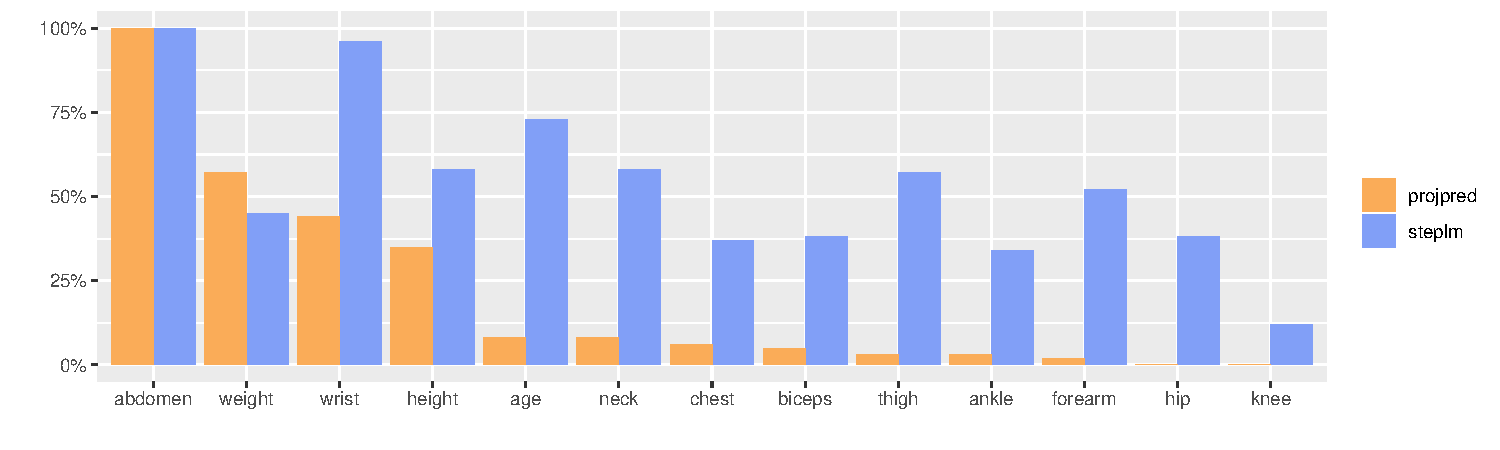
\includegraphics[width=0.98\textwidth]{graphics/inc_prob.pdf}
  \caption{Bootstrap inclusion frequencies after 100 bootstrap samples.}
  \label{fig:inclusion_frequencies}
\end{figure}


\begin{table}[tp]
\scriptsize
\centering
\begin{tabular}{l||l|r||l|r}
  \hline
M & projpred & Freq (\%) & steplm & Freq (\%)  \\ 
  \hline
1 & abdomen, weight & 39 & abdomen, age, forearm, height, hip, neck, thigh, wrist & 4 \\
2 & abdomen, wrist & 10 & abdomen, age, chest, forearm, height, neck, thigh, wrist & 4 \\
3 & abdomen, height & 10 & abdomen, forearm, height, neck, wrist & 2 \\
4 & abdomen, height, wrist & 9 & abdomen, forearm, neck, weight, wrist & 2 \\
5 & abdomen, weight, wrist & 8 & abdomen, age, height, hip, thigh, wrist & 2 \\
6 & abdomen, chest, height, wrist & 2 & abdomen, age, height, hip, neck, thigh, wrist & 2 \\
7 & abdomen, biceps, weight, wrist & 2 & abdomen, age, ankle, forearm, height, hip, neck, thigh, wrist & 2 \\
8 & abdomen, height, weight, wrist & 2 & abdomen, age, biceps, chest, height, neck, wrist & 2 \\
9 & abdomen, age, wrist & 2 & abdomen, age, biceps, chest, forearm, height, neck, thigh, wrist & 2 \\
10 & abdomen, age, height, neck, thigh, wrist & 2 & abdomen, age, ankle, biceps, weight, wrist & 2 \\
   \hline
\end{tabular}
\caption{Bootstrap model selection frequencies after 100 bootstrap samples.}
\label{tab:model_frequencies}
\end{table}


First two rows of Table \ref{tab:model_performances} report the
predictive performances, in terms of cross-validated root mean square
error (RMSE), of the full model and the selected models using either
the projection predictive approach or the stepwise backward
elimination.  There is no difference in predictive performance of the
selected models by different approaches even if there is difference in
the selected features.

We repeat the experiment with a modified data set by adding 84
unrelated noisy features. Last two rows of Table
\ref{tab:model_performances} report cross-validated RMSE, the size of
the selected model and the number of selected noisy features using
either the projection predictive approach or the stepwise backward
elimination.  The projection predictive approach has similar
predictive performance and the same submodel size as in the first
experiment, whereas the stepwise regression has worse predictive
performance and selects a much larger submodel including a large
number of irrelevant features.

\begin{table}[tp]
\scriptsize
\centering
\begin{tabular}{l|r|r|r|r}
  \hline
 & RMSE(Full) & RMSE(Sel) & Size(Sel) & SizeIr(Sel) \\ 
  \hline
projpred & 4.35 & 4.47 & 2 & -  \\
steplm & 4.38 & 4.47 & 7 & - \\
\hline
\hline
projpred & 4.58 & 4.54 & 2 & 0  \\
steplm & 5.89 & 5.43 & 19 & 13 \\
   \hline
\end{tabular}
\caption{Model predictive performances with original data (first two
  rows) and adding noisy features (last two rows) estimated with
  10-fold cross-validation. Abbreviations: Full = full model; Sel =
  selected submodel; Size = total number of included covariates;
  SizeIr = number of included irrelevant covariates.}
\label{tab:model_performances}
\end{table}

Both projpred and steplm compare a large number of models using either
forward or backward search, which can lead to selection induced
overfitting, but even with 100 covariates projpred is able to select a
submodel with similar performance as the full model. Although projpred
uses Bayesian inference and steplm maximum likelihood, it is not
decisive feature explaining the difference in the performance.  The
main difference between the approaches is whether a reference model is
used or not, and in the rest of the paper we look into more detail how
the use of reference model helps and limitations of the approach.

\subsection{Benefits and cost of using a reference model}

A properly designed reference model is able to filter parts of the
noise present in the data, and hence provide an improved and more
stable selection process. This holds even if the reference model does
not perfectly resemble the true data generating process. Moreover, our
analyses indicate that the substantial reduction of variance
attributable to noise is usually more important than small potential
bias due to model misspecification.  We argue that, regardless of how
the reference model is set up and used in the inference procedure, it
can be always seen as acting as a filter on the observed
data. Furthermore, regardless of what specific model selection method
is used, a reference model can be used instead of raw data during the
selection process to improve the stability and selection
performance. Our results indicate that the core reason why the
reference model based methods perform well is the reference model
itself, rather than the specific way of using it.  In general, the
less data we have and the more complex the estimated models, the
higher the benefit of using a reference models as the basis for
variable selection.

If one of the models to be compared is the full model which can be
used as a reference model, there is no additional cost of using a
reference model. Sometimes including all the available features in an
elaborate model can often be computationally demanding.  In such a
case, even simpler screening or dimensionality reduction techniques,
as for example the supervised principal components
\citep{bair2006prediction,piironen2018} can produce useful reference
models.

The remainder of the paper is structured as follows. In Section
\ref{reference-model-approach}, we review the concept of the reference
model, its benefits with examples and how it can be used as a filter
on data in a simple way. In Section \ref{comparison}, we show the
benefits of a reference model approach, regardless of what specific
procedure is applied, using the normal means estimation problem as a
benchmark. Finally, we end with a conclusion in Section
\ref{conclusion}.


\hypertarget{reference-model-approach}{%
\section{Why the reference model helps}\label{reference-model-approach}}
 
A good predictive model is able to filter part of the noise present in
the data. The noise is the main source of the instability and tends to
obscure the relevance of the covariates in relation to the target
variable of interest. Let us consider the following simple
explanatory example taken from \cite{paper:projpred}. The data
generation mechanism is
\begin{alignat}{2} \label{eq:simulated_data}
     &f\sim N(0,1) && \nonumber \\ 
     Y|&f\sim N(f,1) && \\
     X_{j}|&f \overset{iid}{\sim} N(\sqrt{\rho}f,1-\rho) \quad &&j=1,..,k \nonumber \\
     X_{j}|&f \overset{iid}{\sim} N(0,1) &&j=k+1,..,p \nonumber,
\end{alignat}
where $f$ is the latent variable of interest of which $Y$ is a noisy
observation. The first $k$ covariates are strongly related to the
target variable $Y$ and correlated among themselves. Precisely, $\rho$
is the correlation among any pair of the first $k$ covariates, whereas
$\sqrt{\rho}$ and $\sqrt{\rho/2}$ are the level of correlation between
any relevant covariate and, respectively, $f$ and $Y$. If we had an
infinite amount of observations, the sample correlation would be equal
to the true correlation between $X_j$ and $Y$. However, even in this
ideal asymptotic regime, this correlation would still remain a biased
indicator of the true relevance of each covariate (represented by the
correlation between $X_j$ and $f$) due to the intrinsic noisy nature
of $Y$.

When using a reference model, we first obtain predictions for $f$
using all the covariates $\{X_{j}\}_{j=1}^{p}$ taking into account
that we have only observed the noisy representation $Y$ of $f$. If our
model is good, we are able to describe $f$ better than $Y$ itself can,
which improves the accuracy in the estimation of the relevance of the
covariates.  Figure \ref{fig:correlation} illustrates this process in
the form of a scatter plot of (absolute) correlations of the
covariates with $Y$ against the corresponding correlations with the
predictions of a reference model (in this case the posterior
predictive means of model \eqref{eq:ref_mod}; see Section
\ref{simulated-data}). Looking at the marginal distributions, we see
that using a reference model to filter out noise in the data, the two
groups of features (relevant and non-relevant) can be distinguished
much better than when the correlation is computed using the observed
noisy data directly.

\begin{figure}[tp]
  \centering
  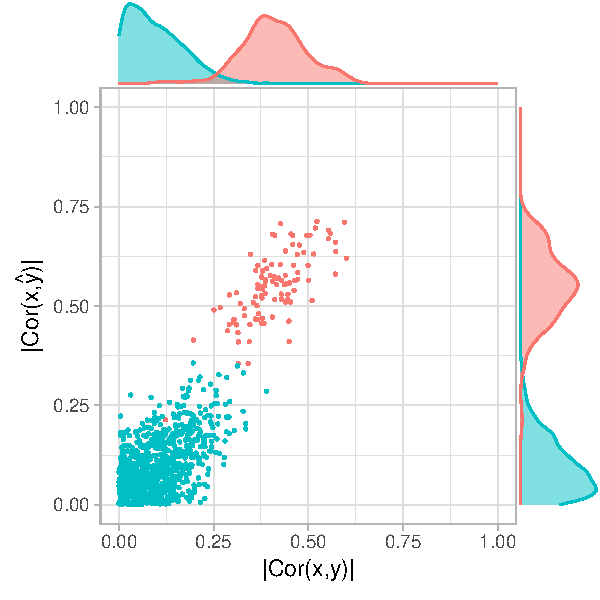
\includegraphics[width=0.3\textwidth]{graphics/correlation.pdf}
  \caption{Sample correlation plot of each feature (relevant in red, 
  non-relevant in blue) with the target variable $y$ and the latent variable 
  $f$ respectively on the x and y axis. Data are generated according to 
  procedure \eqref{eq:simulated_data} with parameters $n=70$, $\rho=0.3$,
  $k=100$, $p=1000$.\\}
  \label{fig:correlation}
\end{figure}

\hypertarget{comparison-minimal-subset}{
\section{A comparison for the minimal subset selection}\label{comparison-minimal-subset}}

Addressing the problem of selecting the minimal subset of relevant/predictive features, 
we compare with a simulation study the selection via projection predictive approach, 
via stepwise forward selection with/without a reference model on top and a Bayesian 
stepwise forward selection.
\begin{itemize}
\item projpred (ref model based): reference model is a linear regression over the first 
five supervised principal components, search heuristics is forward search and the predictive 
performance is estimated via 10-fold cross-validation.
\item stepwise selection (data based): it's based on AIC comparison
\item stepwise selection (ref model based): reference model is a linear regression 
over the first five SPC. The reference model point predictions (posterior predictive means $\hat{y}$) 
are used instead of the target variable values $y$. Based on AIC comparison
\item Bayesian stepwise selection (data based): At each step the model fitted is a 
linear regression using RHS prior and the feature excluded is the one with higher 
Bayesian p-value, defined as:
\begin{equation}
\text{Bayesian p-value}(\theta) := \text{min}\{P(\theta\leq0|D),P(\theta>0|D)\}
\end{equation}
The selection continues if the reduced model has an elpd score higher than the
current fitted model.
\end{itemize}

We simulate data according to \eqref{eq:simulated_data} fixing the overall number of 
features equal to $p=100$ with $k=20$ of them being predictive. In Figure \ref{fig:rmse_vs_fdr} 
it is shown, for different values of $n$ and $\rho$, the predictive performance in terms of 
root mean square error and the false discovery rate of the selected submodel, averaged after 100 data simulations.
Figure \ref{fig:entropy} reports the entropy scores for the different methods compared. Lower entropy corresponds to
a more stable selection. Highly correlated predictive features may happen to be alternately selected, making the measure of
the stability of the selection a non-trivial task. Entropy suffers of such a problem, thus such a measure should be seen
as one of different possible measurements of the actual stability. We note that the reference model approach slightly improves 
with respect to the corresponding data based methods, whereas the projection predictive approach results to be far more stable
than all the other ones.


\begin{figure}[tp]
  \centering
  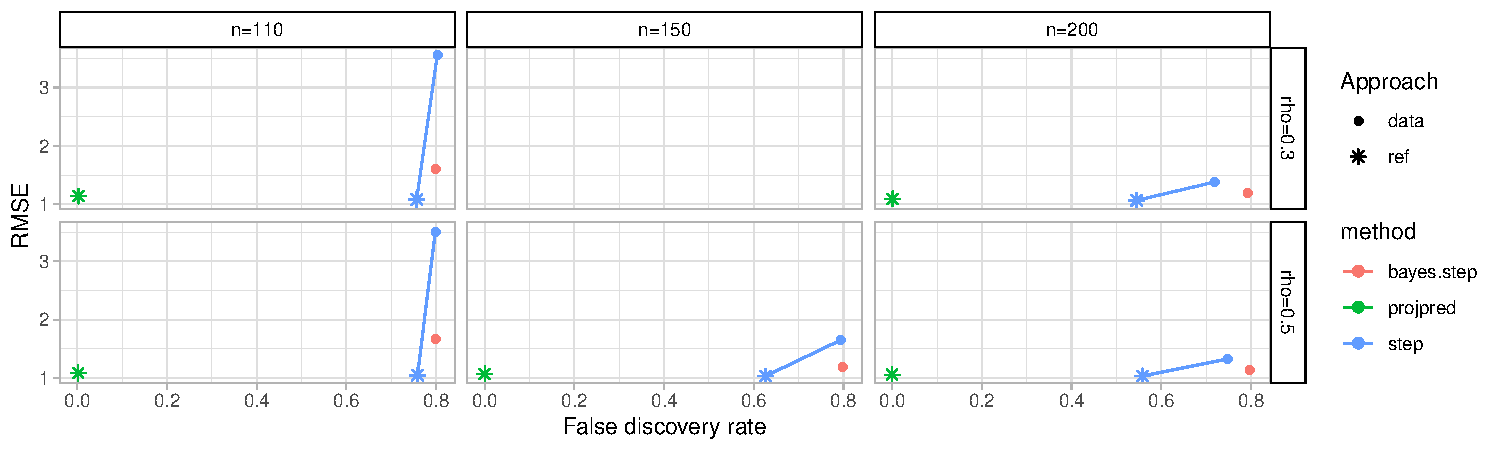
\includegraphics[width=0.98\textwidth]{graphics/rmse_vs_fdr.pdf}
  \caption{Root mean square error (RMSE) against false discovery rate for the minimal subset of feature selection.\\}
  \label{fig:rmse_vs_fdr}
\end{figure}

\begin{figure}[tp]
  \centering
  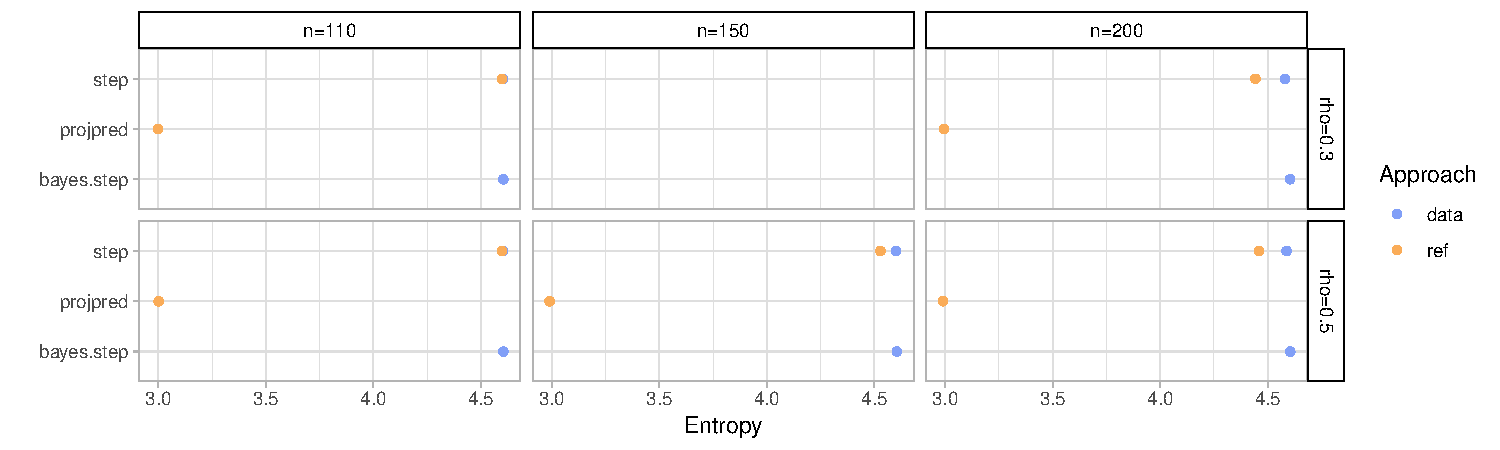
\includegraphics[width=0.98\textwidth]{graphics/entropy.pdf}
  \caption{Entropy score for the minimal subset of feature selection.\\}
  \label{fig:entropy}
\end{figure}



\hypertarget{comparison}{%
\section{A comparison in the normal means problem framework}\label{comparison}}

In this section, we analyse in more detail the benefits of reference
model approaches in combination of a few common variable selection
approach.

\subsection{Simulated data}

The normal means problem consists of estimating the (usually
sparse) vector of means of a vector of normally distributed
observations. The dimensionality of the vector of means is denoted by
$p$ and $\{z_{j}\}_{j=1}^{p}$ is the vector of observations of the
random variables $\{Z_{j}\}_{j=1}^{p}$. The task is to estimate the
latent variables $\{\theta_{j}\}_{j=1}^{p}$ of the following model: \
\begin{equation}\label{eq:normal_means_problem}
Z_{j}|\theta_{j},\sigma\overset{ind}{\sim}N(\theta_{j},\sigma^{2}), \quad j=1,..,p.
\end{equation}
This is equivalent to a linear regression where the design matrix is
the identity matrix with the number of features being equal to the
number of observations. This formulation can be found in practice, for
example, in the analysis of microarray data, where a large set of
genes are tested in two groups of patients labeled as positive or
negative to some disease \citep{paper:efron,efron2012large}. The
objective of the analysis is to select the subset of genes
statistically relevant to the disease. One common way to proceed is to
compute the two-sample $t$-statistic for every gene separately.  After
normalising these statistics, they then become the data, $Z$, in the
normal means problem \eqref{eq:normal_means_problem}. For further
details see the examples in \cite{paper:efron, efron2012large}.

In our experiments, we retrieve the normal means problem from the
sample correlations between the target and the covariates using the
Fisher $z$-transformation \citep{hawkins1989using}. Suppose we have a
continuous target random variable $Y$, a set of $p$ continuous
covariates $\{X_{j}\}_{j=1}^{p}$, and denote
$\rho_{j}=Cor(Y,X_{j})$. Further, suppose we have observed $n$
statistical units and define $r_{j}$ the sample correlation between
the observations of the target variables $\{y_{i}\}_{i=1}^{n}$ and the
$j$-th covariate $\{x_{ij}\}_{i=1}^{n}$. Finally, we refer to the
Fisher $z$-transformation function $\text{tanh}^{-1}(\cdot)$ as
$T_{F}(\cdot)$. Assuming each pair $(Y,X_{j})$ to be bivariate
normally distributed, the corresponding transformed correlations are
approximately normally distributed with known variance: \
\begin{equation} \label{eq:fisher_transformation}
T_{F}(r_{j})\overset{ind}{\sim} N(T_{F}(\rho_{j}),\frac{1}{n-3}) \quad j=1,..,p.
\end{equation}
Therefore, rescaling the quantities $T_{F}(r_{j})$ by $\sqrt{n-3}$ and
denoting the results as $z_{j}$, we have the formulation
\eqref{eq:normal_means_problem} of the normal means problem, this time
with unit variance: \
\begin{equation} \label{eq:normal_means_problem2}
Z_{j}|\theta_{j}\overset{ind}{\sim}N(\theta_{j},1) \quad j=1,..,p.
\end{equation}
Now the quantities of interest $\theta_{j}$ are equal to
$\sqrt{n-3}\,T_{F}(\rho_{j})$.

We use different levels of correlation $\rho\in\{0.3,0.5\}$ and number
observation $n\in\{50,70,100\}$. The total number of covariates $p$
and the number of relevant covariates $k$ are fixed to $p = 1000$ and
$k = 100$, respectively. In general, the lower $\rho$ and $n$, the
more challenging the selection.

\subsection{Model selection approach to be compared}

The Bayesian estimation methods we use to solve the normal means
problem have in common that first a Bayesian regression model is
fitted using some sparsifying prior on the regression coefficients,
for example, as discussed in \cite{paper:dirichlet_laplace},
\cite{bhadra2017horseshoe+} and \cite{johnstone2004needles}.  In our
experiments, we include the Dirichlet-Laplace
\cite[DL;][]{paper:dirichlet_laplace} prior and the regularised
horseshoe (RHS) prior \citep{paper:rhs}, which we think scales better
to higher number of covariates as compared to other horseshoe-like
priors.

% If these priors have continuous support, as is the case for the DL and
% horseshoe-like priors \citep{paper:hs,bhadra2017horseshoe+,paper:rhs},
% there is no canonical way to complete the selection since the
% posterior probability of an exactly zero signal is always
% zero. Whereas \cite{paper:dirichlet_laplace} used k-means clustering
% over the posterior samples to perform the actual selection,
% \cite{bhadra2017horseshoe+} just focused their analysis on the
% obtained shrinkage and the correct estimation of the sparse signals
% without any actual selection.

% For the Bayesian regression
% models with these priors, we compare the posterior shrinkage and the
% correct estimation of the sparse signals with and without using a
% reference model as a noise filter. For this purpose, we consider the
% average SSE (sum of square errors) and the average SESE (sum of
% expected square errors) as quantities measuring estimation
% accuracy. They are defined as \
% \begin{align}
% \text{SSE}&=\frac{1}{n-3}\sum_{j=1}^{p}(\hat{\theta}_{j} - \theta^{0}_{j})^{2} \label{eq:SSE} \\
% \text{SESE}&=\frac{1}{n-3}\sum_{j=1}^{p}\int_{\mathbb{R}}(\theta_{j}-\theta^{0}_{j})^{2}p(\theta_{j}|z_{1},..,z_{p})d\theta_{j} \\
% &=\frac{1}{n-3}\sum_{j=1}^{p}\mathbb{E}_{\theta_{j}}[(\theta_{j}-\theta^{0}_{j})^{2}|z_{1},..,z_{p}], \label{eq:SESE}
% \end{align}
% where $\theta_{j}^{0}=\sqrt{n-3}\,T_{F}(\rho_{j})$ is the true value,
% $\hat{\theta}_{j}$ is the posterior median of each parameter
% $\theta_{j}$. We divide the errors by $(n-3)$ to have quantities
% independent of the number of statistical units.  The SESE takes the
% posterior uncertainty in account and thus also the shrinkage of the
% posterior distributions, whereas the SSE only measures the bias in the
% point estimates.  Any (sensible) point estimate could be used to
% compute the SSE but here we follow \cite{paper:dirichlet_laplace} and
% use the posterior median. The results that we show later on in Section
% \ref{shrinkage-signal} are not sensitive to the choice of this point
% estimate.

% For shrinkage priors, one central aspect is the amount of shrinkage
% they actually impose on the relevant and irrelevant features. Ideally,
% the irrelevant features should be completely shrunk to zero while the
% relevant features should not be shrunk at all. The amount of shrinkage
% can be quantified by the shrinkage factor $\kappa_{j}$ for each
% parameter $\theta_{j}$ ranging from $0$ (no shrinkage) to $1$
% (complete shrinkage). For model \eqref{eq:normal_means_problem2} with
% a hierarchical shrinkage prior of the type
% \begin{align}
% Z_{j}|&\theta_{j}\overset{ind}{\sim}N(\theta_{j},1) \qquad j=1,..,p \\
% &\theta_{j}|\tau,\nu_{j}\overset{ind}{\sim}N(0,\nu_{j}^{2}\tau^{2})
% \end{align}
% the shrinkage factor $\kappa_{j}$ is defined as
% \begin{equation}
% \kappa_{j}=\frac{1}{1+\tau^{2}\nu_{j}^{2}}.
% \end{equation}
% \
% For RHS and DL priors we have
% \begin{equation}
% \kappa_{j}^{\text{RHS}}=\frac{1}{1+\tau^{2}\lambda_{j}^{2}}, \qquad \kappa_{j}^{\text{DL}}=\frac{1}{1+\psi\phi_{j}^{2}\tau^{2}}.
% \end{equation}
% In the left hand-side expression, $\tau$ and $\lambda_{j}$ represent
% the global and local shrinkage parameters of the regularised horseshoe
% prior \cite[for further details see][]{paper:rhs}, whereas on the
% right hand-side, $\psi\phi_{j}^{2}\tau^{2}$ is the variance term of
% the Dirichlet-Laplace prior of parameter $\theta_{j}$ following the
% notation of \cite{paper:dirichlet_laplace}. We use the posterior mean
% of $\kappa_{j}$ as a point estimate.

Within the set of complete selection procedures, we consider three
Bayesian methods.  \cite{johnstone2004needles} use a spike-and-slab
type prior given by a mixture of a delta distribution in zero and a
heavy-tailed distribution \cite[see
also][]{paper:spike_slab_mitchell}. When the latter is a Laplace
distribution, they show an interesting thresholding property of the
median estimator and, based on this observation, present a complete
selection procedure using their prior. We refer to this method as
EB.med. Further, we use a method to control for the local false
discovery rate (loc.fdr) as described in \cite{paper:efron,
  efron2012large}. Finally, we device a simple selection procedure
based on posterior credible intervals using the regularised horseshoe
prior in which we select covariates whose 90\% credible intervals
excludes zero (ci.90). All of these methods provide a complete
selection procedure and we compare their performance with and without
using a reference model on top of them. As criteria of selection
performance, we evaluate the average false discovery rate (i.e., the
ratio of the number of non-relevant selected features over the number
of selected features) and the average sensitivity (i.e., the ratio of
the number of relevant selected features over the total number of
relevant features). We also provide a comparison of the stability of
the selection by means of a stability measure proposed by
\cite{paper:stability}. Table \ref{tab:comparison} summarises the
methods used in the numerical experiments.

\begin{table}[tp]
\scriptsize
\centering
\begin{tabular}{l|l|l|l}
 Method & Abbreviation & Type & Quantities of interest \\ 
  \hline
 Regularised Horseshoe & RHS & Shrinkage prior & SSE, SESE, $\kappa$ \\
 Dirichlet-Laplace & DL & Shrinkage prior & SSE, SESE, $\kappa$ \\
 Local false discovery rate & loc.fdr & Complete selection & fdr, sensitivity, stability \\
 Median estimator & EB.med & Complete selection & fdr, sensitivity, stability \\
 Credible intervals & ci.90 & Complete selection & fdr, sensitivity, stability \\
\end{tabular}
\caption{Summary of the shrinkage and selection methods used in the numerical experiments.}
\label{tab:comparison}
\end{table}

\hypertarget{simulated-data}{%
\subsection{Simulated data}\label{simulated-data}}

Here we use simulated data in order to control the difficulty of the
selection problem. We rely on the scheme \eqref{eq:simulated_data}
using different levels of correlation $\rho\in\{0.3,0.5\}$ and number
observation $n\in\{50,70,100\}$. The total number of covariates $p$
and the number of relevant covariates $k$ are fixed to $p = 1000$ and
$k = 100$, respectively. In general, the lower $\rho$ and $n$, the
more challenging the selection. As mentioned, this data generation
mechanism was originally proposed by \cite{paper:projpred} who also
devise a reference model performing sufficiently well in this
situation. It consists of a linear regression using the first five
supervised principal components (SPCs) \citep{bair2006prediction,
  piironen2018} as covariates and imposing an hierarchical prior on
their coefficients: \
\begin{equation}
\label{eq:ref_mod}
\begin{aligned}
    Y_{i}|&\boldsymbol{\beta},\sigma^{2},\boldsymbol{u}_{i} \overset{ind}{\sim} N(\boldsymbol{u}_{i}^{T}\boldsymbol{\beta},\sigma^{2}) \quad &i=1,..,n \\
    &\beta_{j}|\!\begin{aligned}[t] &\tau \overset{iid}{\sim} N(0,\tau^{2})\\
    &\tau \sim t_{4}^{+}(0,s_{max}^{-2}) 
    \end{aligned} &j=1,..,5 \\ 
    &\sigma \sim t_{3}^{+}(0,10). \\
\end{aligned}
\end{equation}
In the above, $u_{ij}$ represents the $j$-th SPC evaluated at
observation $i$, and $s_{max}$ denotes the sample standard deviation
of the largest SPC.  The SPCs are computed through the
\texttt{R}-package \texttt{dimreduce} setting the screening threshold
parameter at $0.6s_{max}$.  In our experiments the results are not
sensible to such a choice of the screening threshold, yet a more
principled approach would be to use cross-validation to select the
threshold as done in \cite{paper:projpred}.

The normal means problem formulation is obtained as explained in
Section \ref{comparison} by applying the Fisher-z-transformation to
the empirical correlations. We label the reference approach as
``ref'', which consists of using the reference model on top of the
computation of the z-values, and the standard approach based on the
observed data simply as ``data''. In Section \ref{shrinkage-signal},
we analyse the different shrinkage and signal estimates in the context
of the full Bayes estimation methods by comparing the ref and data
approach. In Section \ref{complete-selection}, we present results for
the complete selection procedures.

% \hypertarget{shrinkage-signal}{%
% \subsubsection{Shrinkage and signal analysis}\label{shrinkage-signal}}
% In the framework of fully Bayesian estimation methods, we analyse the
% effect of the reference model using two continuous hierarchical
% shrinkage priors: the Dirichlet-Laplace
% \citep{paper:dirichlet_laplace} and the regularised horseshoe prior
% \citep{paper:rhs}.
% %
% For the Dirichlet hyperparameter of the Dirichlet-Laplace prior, we
% use an uniform prior on the interval $(1/p,1/2)$. For the regularised
% horseshoe prior, we follow the recommendations provided in
% \cite{paper:rhs} by setting the prior guess of the number of relevant
% covariates to one in order to achieve the highest possible
% shrinkage. The results are not sensitive with respect to the specific
% choice.  \ Since, as explained at the start of Section
% \ref{comparison}, continuous priors usually do not provide an
% automatic selection procedure, we study the amount of shrinkage and
% the bias of the posterior medians looking at the SESE and the SSE (see
% definitions \eqref{eq:SSE} and \eqref{eq:SESE}), together with the
% posterior mean of the shrinkage factors.

% \begin{figure}[tp]
%   \centering
%   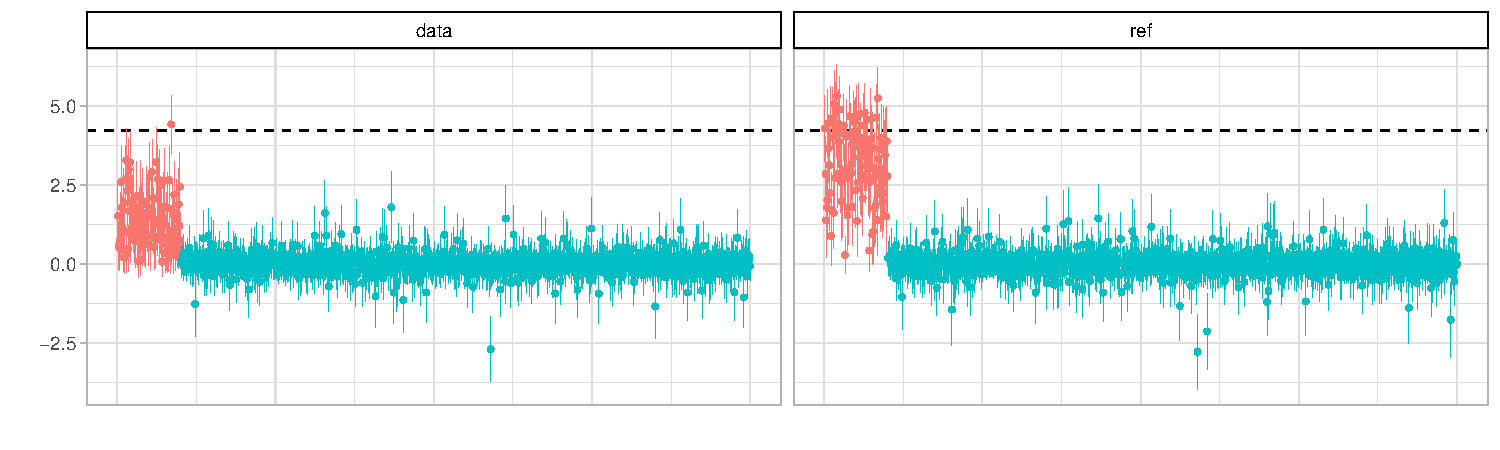
\includegraphics[width=0.98\textwidth]{graphics/post_int.pdf}
%   \caption{Posterior intervals for the parameters of the normal means
%     problem ($n=50$, $\rho=0.3$) using the regularised horseshoe
%     prior. Posterior means and one standard deviation intervals are
%     depicted. Relevant and non-relevant features are displayed in red
%     and in blue respectively. Horizontal dashed lines corresponds to
%     the true value of the mean for the relevant features.\\}
%   \label{fig:posterior_intervals}
% \end{figure}

% Figure \ref{fig:posterior_intervals} shows an example of posterior
% distributions for the model \eqref{eq:normal_means_problem2} using the
% regularised horseshoe prior with the data approach on the left and the
% ref approach on the right-hand side. It is evident how the reference
% model helps in tearing apart the signal from the noise, resulting in
% less biased estimates and clearer separation between relevant and
% irrelevant features. This is quantified in Figure \ref{fig:SESE_SSE}
% where average SESE and SSE are depicted based on 100 simulations. We
% observe that the reference approach (in orange) has a clearly lower
% estimate for both the SESE and the SSE. As $n$ and $\rho$ increase,
% the amount of error diminishes, as expected, due to a larger amount of
% information of the relevance of each variable provided by the
% data. The two priors (RHS and DL) seem to achieve similar results
% under all conditions.

% \begin{figure}[tp]
%   \centering
%   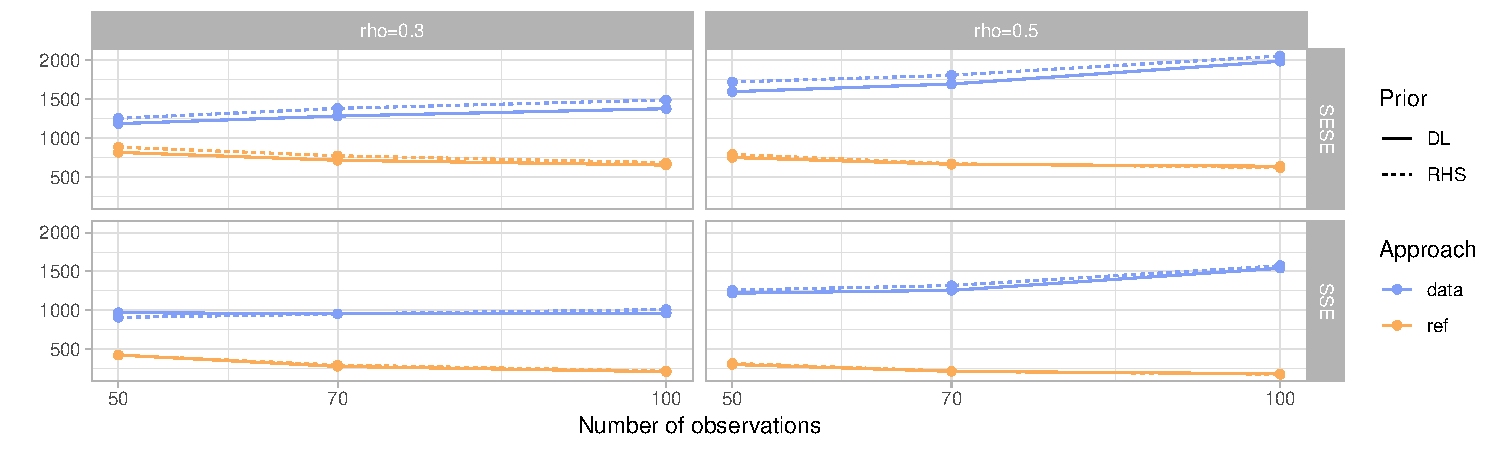
\includegraphics[width=0.98\textwidth]{graphics/SESE_SSE.pdf}
%   \caption{Average SESE and SSE with one standard deviation intervals based on 100 simulations.\\}
%   \label{fig:SESE_SSE}
% \end{figure}

% Figure \ref{fig:k} shows the posterior means for the shrinkage factors
% of each parameter using the regularised horseshoe prior, averaged over
% 100 data simulations. Relevant and non-relevant features are
% highlighted in red and blue respectively. The ideal shrinkage would be
% $\kappa=0$ when the parameter is a signal and $\kappa=1$ when it is
% noise. The shrinkage factors using the data and reference approach are
% depicted on the y-axis and on the x-axis respectively. If the
% reference model did not make any difference, we would expect the
% points to lie on the diagonal. For the non-relevant features points
% are on the diagonal on average for all the simulated scenarios, which
% implies that their shrinkage was not improved by the reference
% approach. For the relevant features, the points are always located
% under the diagonal, which means that the reference model helps and
% true signals are shrunk less. This benefit is roughly proportional to
% the difficulty of the problem, that is, the benefit increases with
% lower correlations and a smaller number of observations. The perfect
% distinction of the two clusters of features (relevant and
% non-relevant) observable on both the marginal distributions of the
% shrinkage factors is due to the averaging over the 100 data
% simulations. In a single data realisation, there is more noise and the
% cluster are closer and overlapping. The results for the
% Dirichlet-Laplace prior are very similar.

% \begin{figure}[tp]
%   \centering
%   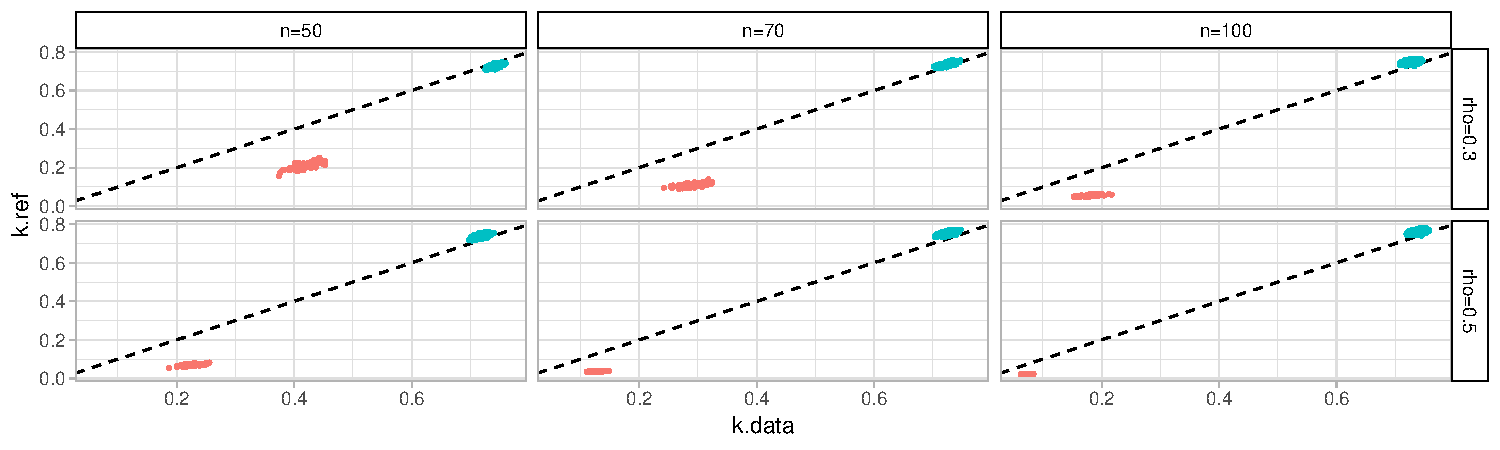
\includegraphics[width=0.98\textwidth]{graphics/k_RHS.pdf}
%   \caption{Average posterior mean values for the shrinkage factors
%     using the regularised horseshoe prior based on 100
%     simulations. Relevant and non-relevant variables are displayed in
%     red and blue respectively.\\}
%   \label{fig:k}
% \end{figure}


\hypertarget{complete-selection}{%
\subsubsection{Complete selection analysis}\label{complete-selection}}
As complete selection procedures we consider the control of the local
false discovery rate \citep{paper:efron, efron2012large}, the
empirical Bayes median \citep{johnstone2004needles}, the selection
by posterior credible intervals and an adaptation of the projection 
predictive approach that we name iterative projection.\

The control of the local false discovery rate is applied through the
\texttt{R}-package \texttt{locfdr}. It consists of testing the
z-values $\{z_{j}\}_{j=1}^{p}$ on whether they belong to the
theoretical null distribution $f_{0}$ (i.e., the null hypothesis $H_0$
meaning no relevance) against the alternative hypothesis distribution
$f_{1}$. In our case $f_{0}$ corresponds to the standard normal
distribution (see expression \eqref{eq:normal_means_problem2}). The
quantity of interest is the local false discovery rate (loc.fdr)
defined as: \
\begin{equation}
\text{loc.fdr}(z)=P(H_{0}|z)=\frac{f_{0}(z)\pi_{0}}{f(z)},
\end{equation}
where $\pi_{0}$ is the prior probability of $H_0$ and
$f(z)=\pi_{0}f_{0}(z)+(1-\pi_{0})f_{1}(z)$ is the marginal
distribution of the z-values. The latter is estimated using splines
with 7 degrees of freedom. We select features with local false
discovery rate below $0.2$, which is suggested by
\citet{efron2012large} as it corresponds to a Bayes factor larger than
36 (assuming $\pi_{0}\geq0.9$). The results of the comparison are not
sensitive to the specific value. We use the default setting to
estimate $\pi_{0}$ from the data provided by the package.

The empirical Bayes median procedure is given by the
\texttt{R}-package \texttt{EbayesThresh} and consists of fitting a
Bayesian model with a prior composed by a mixture of a delta in zero
and a heavy-tailed distribution. As suggested by
\cite{johnstone2004needles}, we use a Laplace distribution resulting
in a thresholding property, that is, there exists a threshold value
such that all the data under that threshold have posterior median
equal to zero. Therefore the selection is done by selecting only those
parameters whose posterior median is different from zero. The
hyperparameter of the Laplace distribution and the mixing weight of
the prior are estimated by marginal maximum likelihood.  

The selection
by 90\% posterior credible intervals is done using the regularised
horseshoe prior and selecting those features whose posterior
distribution does not include zero in the interval between the 5\% and
the 95\% quantiles.

The iterative projection is a tentative to adapt the projection predictive 
approach to select the whole set of relevant features. Applying the straightforward 
implementation of projpred, we are able to select a minimal subset of features, which
yield to a model with a predictive performance comparable to the full model one.
The iterative projection repeats the projpred selection for different iterations, at each time
excluding from the search path the features selected in the previous steps. At each iteration
the selected submodel size corresponds to the one having a predictive performance close enough
to the baseline model, which in this iterative version is the submodel with the highest predictive
score explored at the current iteration. The stopping rule that we adopted is the following:
\begin{equation} 
\label{eq:rule_of_thumb}
\text{min} \{i\in \{0,..,p\}: \text{P}(\text{elpd}_{i}-\text{elpd}_{\text{best}}>0)\geq \alpha \}
\end{equation}
where $i$ indexes the submodel size and ``best'' stays for the best predictive explored submodel
at the considered iteration. The algorithm terminates when the empty model (only intercept) satisfies
the stopping rule.
The choice of the hyperparameter $\alpha$ can be non-trivial, we have 
observed sensitivity of the selection to such a choice mainly when using cross-validation with a small
number of observations or not very predictive features. 
In our experiments we chose the default value used in the \texttt{projpred} 
\texttt{R}-package that corresponds to $\alpha=0.16$.
\hl{NOTE: if necessary I can add a pseudo-code illustration of the iterative projection algorithm, as 
I did in the thesis}


Figure \ref{fig:sensitivity_vs_fdr_iterated} reports the average sensitivity on
the vertical axis versus the average false discovery rate on the
horizontal axis based on 100 data simulations for the different
combinations of $n$ and $\rho$. For each method (different colours)
the squares and the circles correspond to using the reference and
approach respectively. The best selection performance is on the
top-left corner of each plot, as it implies the lowest false discovery
rate and the highest sensitivity. We see that regardless of the
applied selection method, the use of a reference model improves the
selection performance as it reduces the false discovery rate (shifting
to the left) or increases the sensitivity (shifting upwards). In
accordance with what can be expected, the larger number of
observations and the higher the true correlations, the easier the
selection is. Thus, for easier selection scenarios, the benefits of
the reference model are smaller since the raw data already provide
enough information to identify the relevant covariates. The iterative
projection performs fairly well if the number of observations and the correlation level
are not too small. In those cases it mainly results to be too conservative, resulting in a low
sensitivity, but good false discovery rate. Tuning $\alpha$ might lead to improved selection, yet
the main source of poor performance could well be the miscalibration of the uncertainty of the predictive
utility score for misspecified models with cross-validation \hl{(maybe add some references?)}.


\begin{figure}[tp]
  \centering
  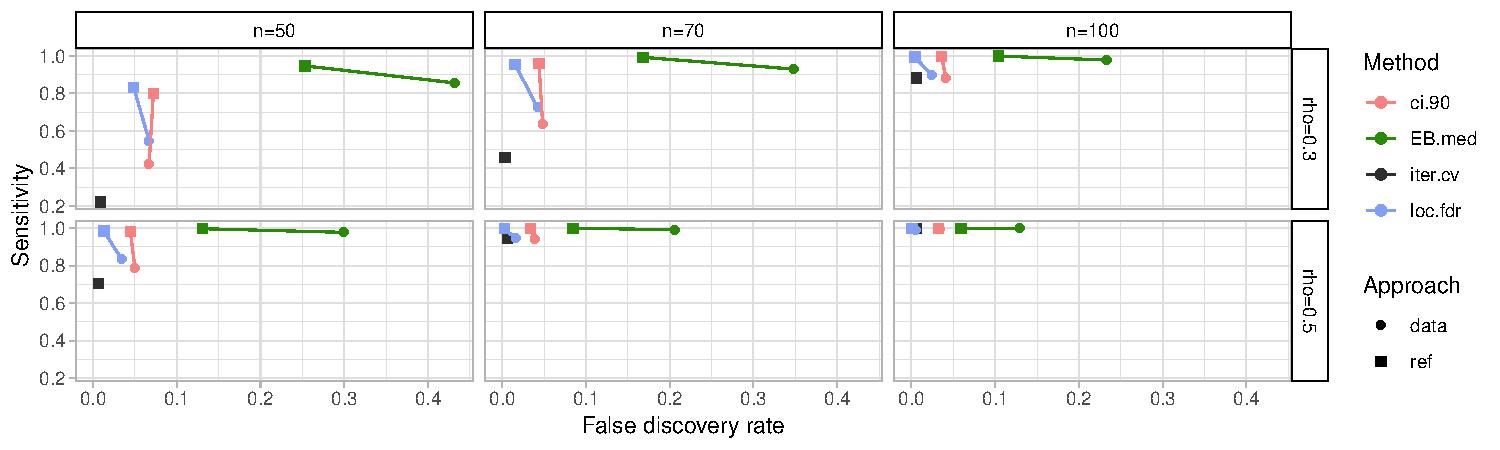
\includegraphics[width=0.98\textwidth]{graphics/sensitivity_vs_fdr_iterated.pdf}
  \caption{Sensitivity against false discovery rate based on 100 data simulations.\\}
  \label{fig:sensitivity_vs_fdr_iterated}
\end{figure}

%\begin{figure}[tp]
%  \centering
%  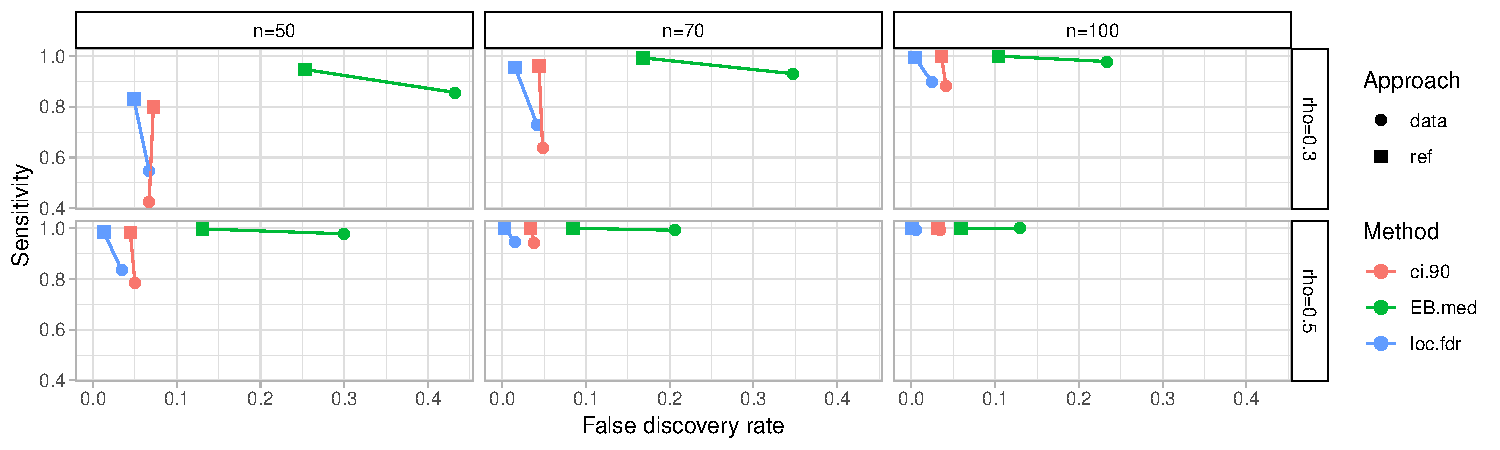
\includegraphics[width=0.98\textwidth]{graphics/sensitivity_vs_fdr.pdf}
%  \caption{Sensitivity against false discovery rate based on 100 data simulations.\\}
%  \label{fig:sensitivity_vs_fdr}
%\end{figure}

Figure \ref{fig:stability_iterated} shows the estimates of the stability
measure proposed by \cite{paper:stability} with 0.95 confidence
intervals based on 100 simulations. Such a measure takes in account
the variability of the subset of the selected features at each
simulation (originally at each bootstrap sample), modelling the
selection of each variable as a Bernoulli process. Further details are
available in \cite{paper:stability}. The reference model helps in
improving the stability of the selection: Again, the benefits are
bigger when the problem is more difficult (small $n$ and $\rho$). In
addition, we observe less uncertainty in the stability estimates for
the reference approach (i.e., smaller width of the 95\% intervals),
which can be still connected to the overall stability of the
procedure. As in Figure \ref{fig:sensitivity_vs_fdr_iterated}, the iterative
projection does not perform well in the hardest scenarios. 

\begin{figure}[tp]
  \centering
  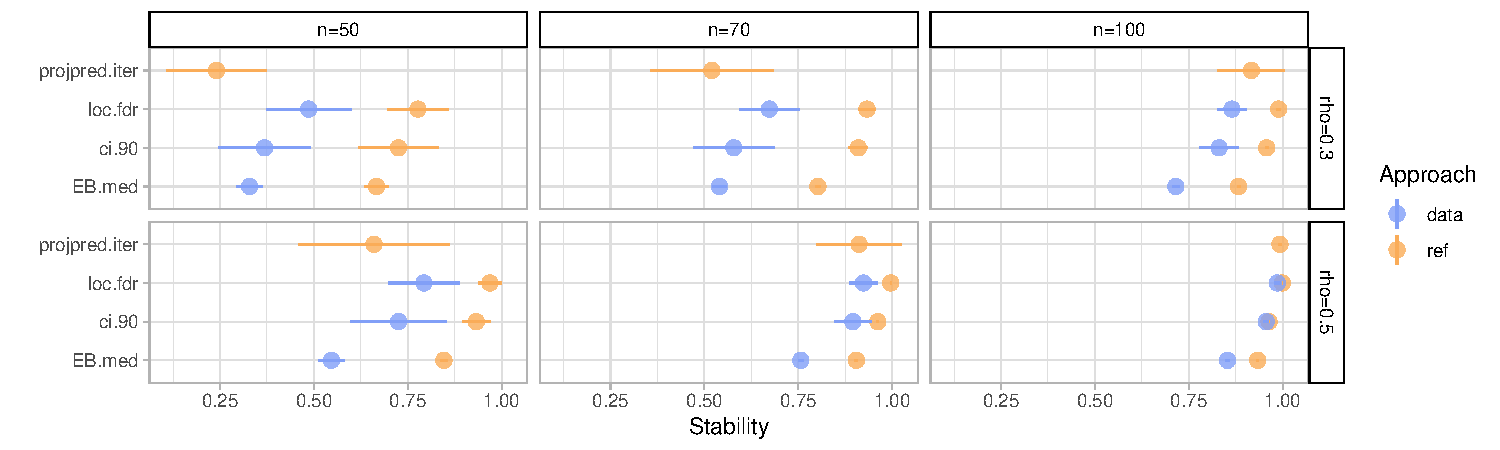
\includegraphics[width=0.98\textwidth]{graphics/stability_iterated.pdf}
  \caption{Stability estimates with 95\% intervals based on 100 data simulations.\\}
  \label{fig:stability_iterated}
\end{figure}


\hypertarget{real-world-data}{%
\subsection{The body fat data: A real world example}\label{real-world-data}}

We conclude our experiments using the real world `body fat' dataset
one more time, which was already described in the motivational example
comparing the projection predictive approach and the stepwise
regression in Section \ref{projection}. We carry out two different
analyses: one using the normal means problem framework and another one
using selection via stepwise backward regression. In the former, we
add noisy uncorrelated covariates to the original data up to a total
of 1000 features. These covariates are normally distributed and scaled
as the original covariates. We compute correlations between each
variable and the target variable, that is the amount of fat, and
transform them by Fisher-Z-transformation. The original assumption in
order for \eqref{eq:fisher_transformation} to hold is that the
variables are jointly normally distributed. In our experience the
normal approximation in \eqref{eq:fisher_transformation} is still
reasonable, but after rescaling by $\sqrt{n-3}$ we do not fix the
variance to be one, and instead estimate it from the data. The methods
we compare are those used in Section \ref{complete-selection}: the
control of the local false discovery rate (loc.fdr), the empirical
Bayes median (EB.med) and the selection by posterior credible
intervals at level 90\% (ci.90).  In order to vary the difficulty of
the selection, we bootstrap subsamples of different sizes, going from
$n=50$ up to $n=251$ (i.e., the full size of the data). For each
condition, results are averaged over 100 bootstrap samples of the
respective size.

\begin{figure}[tp]
  \centering
  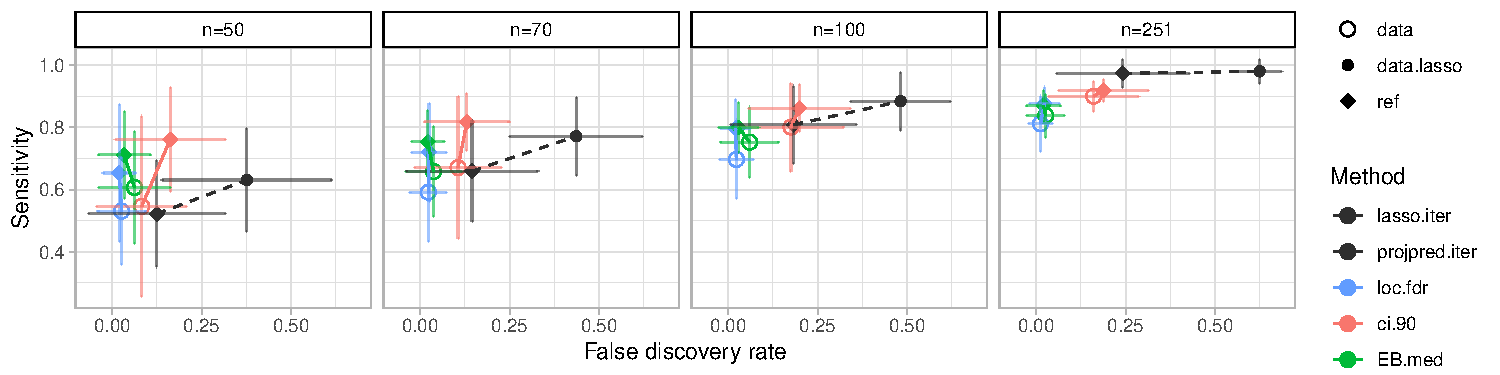
\includegraphics[width=0.98\textwidth]{graphics/bodyfat_sensitivity_vs_fdr.pdf}
  \caption{Sensitivity against false discovery rate based on 100 bootstrap samples.\\}
  \label{fig:bodyfat_sensitivity_vs_fdr}
\end{figure}

\begin{figure}[tp]
  \centering
  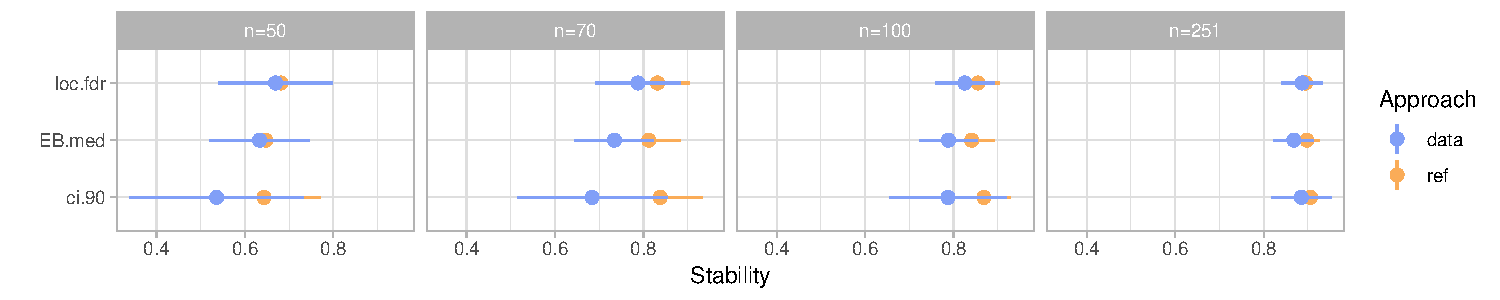
\includegraphics[width=0.98\textwidth]{graphics/bodyfat_stability.pdf}
  \caption{Stability estimates with 0.95 confidence intervals based on 100 bootstrap samples.\\}
  \label{fig:bodyfat_stability}
\end{figure}

Figure \ref{fig:bodyfat_sensitivity_vs_fdr} shows the sensitivity
against the false discovery rate. Since we do not have a ground truth
available with regard the original covariates of the data, we believe
it is reasonable to consider all of them relevant, at least at some
degree. The artificially added features are naturally irrelevant by
construction. In almost all the bootstrapped subsamples, the reference
model improves the selection both in terms of sensitivity and false
discovery rate. When $n=50$, we observe a worsening in terms of false
discovery rate, yet by a lower amount compared to the gain in
sensitivity. Again, we observe that the benefits are more evident as
the selection becomes more challenging (i.e., lower number of
observations). Figure \ref{fig:bodyfat_stability} shows the stability
results, still using the measure provided by
\cite{paper:stability}. The benefits of the reference model are here
marginal with only small improvements.

\begin{figure}[tp]
  \centering
  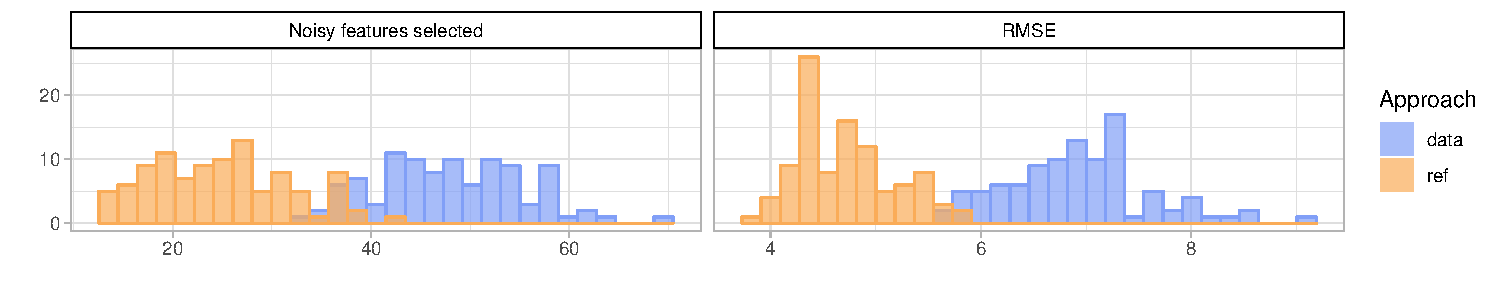
\includegraphics[width=0.98\textwidth]{graphics/bodyfat_step_refvsdata.pdf}
  \caption{Stepwise backward selection with and without using a reference model. The x-axis denotes the number of selected irrelevant features on the left and the out-of-sample RMSE on the right-hand side based on 100 bootstrap samples.\\}
  \label{fig:bodyfat_step_refvsdata}
\end{figure}

In the second analysis, we repeat the selection of Section
\ref{projection} via stepwise backward regression. In this case, the
overall number of covariates (original plus noisy) is 100, as it was
in the last part of Section \ref{projection}. We compare results with
and without using a reference model on top of the procedure following
our simple reference model approach outlined in
\eqref{eq:ref_mod}. Figure \ref{fig:bodyfat_step_refvsdata} shows the
number of irrelevant features included in the final model and the
out-of-sample root mean square error (RMSE). Results are based on 100
bootstrap samples on the whole dataset, and the predictive performance
is tested on the observations excluded at each bootstrap sample. We
observe that the reference model reduces the number of irrelevant
features included in the final model. This leads to less overfitting
and thus to improved out-of-sample predictive performance in terms of
RMSE. The reference model approach applied to the stepwise backward
regression achieves outstanding improvements considering its
simplicity, yet it does not reach the goodness of more thoughtful
implementations, for instance, the projective prediction approach (see
results of Section \ref{projection}).

In this example, we have still used the reference model defined as a
linear regression over some supervised principal components, because
of its fairly good predictive performance and efficient estimation. We
do not argue that this is always a good choice and more sophisticated
models can lead to even better results. Since, in our case, the sake
of the analysis was only to motivate the use of reference models in
general, and since we needed to average results over a lot of
repetitions per simulation condition, we preferred to stick to such a
comparably simple reference model.


\hypertarget{conclusion}{%
\section{Conclusion}\label{conclusion}}

In this paper, we demonstrated the benefits of using a reference model
to improve feature selection, or more generally, model reduction. The
goal of this paper is not to provide a specific procedure to carry out
the selection, but rather to explain and motivate the general benefits
of a reference model.  We have seen how the reference model acts as an
approximation of the data generation mechanism through its predictive
distribution. Such approximation is generally less noisy than the
sample estimation available purely from the observed data, leading to
the main benefits of the reference model approach. In our comparisons,
we have analysed the effect of a reference model in the form of a
filter on the observed target values on top of different widely used
variable selection methods. Overall, using a reference model leads to
more accurate and stable selection results independently of the
specific selection method. These benefits apply to a large family of
different approaches all involving a reference model in one way or the
other. Some of these approaches have been present in the literature
for several years \cite[e.g. see][]{vehtari2012survey,paper:projpred}
but often without a clear explanation of \emph{why} they are actually
favourable and how they connect to other related approaches. We hope
that the present paper can fill some of these gaps by providing a
unifying framework and understanding of reference models.

We argue that, whenever it is possible to come up with a reasonable
reference model, it should be employed on top of the preferred
selection procedure or as an integral part of more complex methods,
for example, the projective prediction approach
\citep{paper:projpred}. Note that one of the main challenges in many
real world application will consist in devising a sensible reference
model itself and assessing its predictive performance. We did provide
a generic way to build simple reference models, but those may not
necessarily be appropriate in all situations. If more sophisticated
reference models are required, which are more specifically tuned to
the data and problem at hand, we recommend them to be developed using
a robust (Bayesian) modelling workflow, for instance, as outlined in
\cite{gabry2019visualization}.
\\

All Bayesian models used in the this paper have been implemented in
the probabilistic programming language \texttt{Stan}
\citep{paper:stan} and fit via dynamic Hamiltonian Monte Carlo
\citep{hoffman2014no,betancourt2017conceptual}. The code to run all
the experiments is available on GitHub
(\url{https://github.com/fpavone/ref-approach-paper}).




 
\bibliography{ref_approach}

%\appendix

%\hypertarget{ap:shrinkage_signal}{%
%\section{Appendix: Shrinkage factors with Dirichlet-Laplace prior}\label{ap:shrinkage_signal}}
%Figure \ref{fig:k_DL} shows the posterior mean shrinkage factors using the Dirichlet-Laplace prior for the normal means problem in the simulated data study of Section \ref{comparison}. The result is qualitatively equal to the regularised horseshoe prior's one (see Figure \ref{fig:k}). 

%\begin{figure}[tp]
%  \centering
%  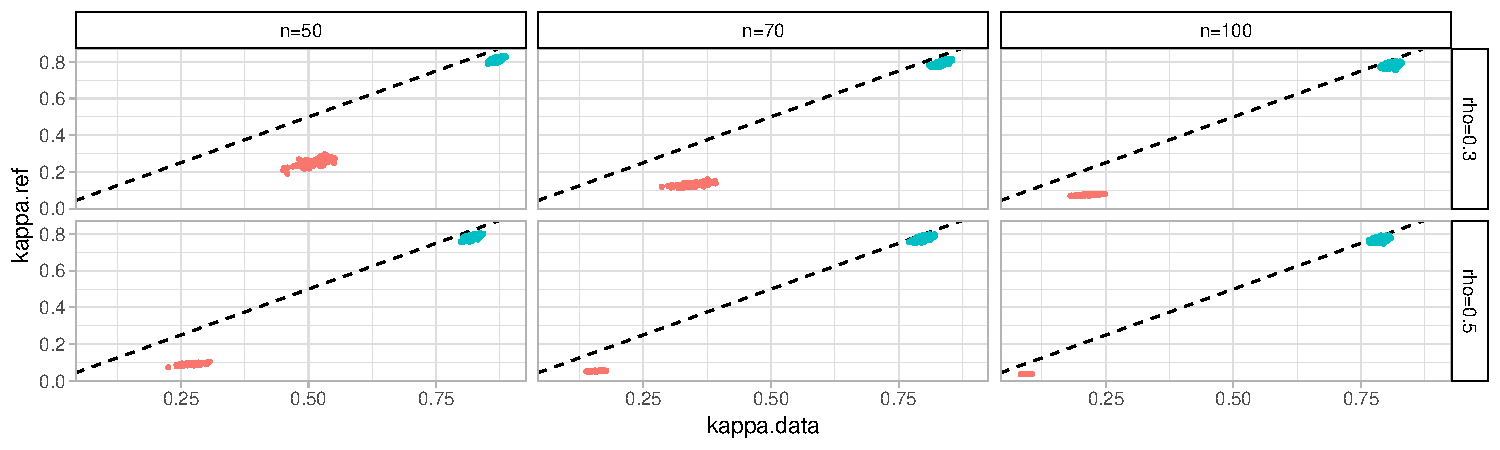
\includegraphics[width=0.98\textwidth]{graphics/k_DL.pdf}
%  \caption{Average posterior mean values for the shrinkage factors using the Dirichlet-Laplace prior based on 100 simulations. Respectively in red and in blue relevant and non-relevant variables.\\}
%  \label{fig:k_DL}
%\end{figure}


As an another example, let us consider a candidate submodel in a
feature selection process and let us refer to the parameter
distribution of the submodel by $\pi$ and to the induced predictive
distribution by $q_{\pi}(\tilde{y})$. We would like to choose $\pi$ so
that $q_{\pi}(\tilde{y})$ maximises some predictive performance
utility, for example, the expected log-predictive density (elpd)
defined as: \
\begin{equation}\label{eq:elpd}
\text{elpd}[q_{\pi}]=\int \text{log}\,q_{\pi}(\tilde{y})p_{t}(\tilde{y})d\tilde{y},
\end{equation}
where $p_{t}(\tilde{y})$ denotes the (usually unknown) true generating
mechanism of future data $\tilde{y}$. If we refer to the posterior
predictive distribution of a reference model with $p(\tilde{y}|D)$,
where $D$ stands for the data on which we conditioned on, we can
approximate \eqref{eq:elpd} using $p(\tilde{y}|D)$ instead of the true
data generation mechanism $p_{t}(\tilde{y})$. The maximisation of the
elpd using the reference model predictive distribution is equivalent
to the minimisation of the Kullback-Leibler (KL) divergence from the
reference model's predictive distribution to the submodel's predictive
distribution: \
\begin{equation} \label{proj_as_filter}
\underset{\pi}{\text{max}} \; \int \text{log}\,q_{\pi}(\tilde{y})p(\tilde{y}|D)d\tilde{y} \leftrightarrow \underset{\pi}{\text{min}} \; \text{KL}[p(\tilde{y}|D)||q_{\pi}(\tilde{y})] 
\end{equation}
The term on the right-hand side of Equation \eqref{proj_as_filter}
describes what is referred to as the projection of the predictive
distribution, which is the general idea behind the projection
predictive approach \cite[see][]{paper:projpred}. Again the reference
model is acting as a filter, or substitute, on data.


Relying on the idea of the reference model as a noise-filter, a
generic reference model approach, which can be used on top of any
feature selection procedure, consists of simply substituting the
target observations with corresponding point predictions of the
reference model, for instance, the posterior predictive
means. Afterwards, any method for feature selection can be used. We do
not argue that such a reference model approach should necessarily be
used as is for feature selection in real applications. There are
several more sophisticated reference model approaches available in the
literature \cite[see,
e.g.][]{paper:projpred,paananen2017variable,paul2008preconditioning},
which are likely to yield even better results. Rather, the reason for
focusing on this simple version is to enable a fair comparison between
a reference model and a purely data based approach when otherwise
using the same selection procedures. Other kinds of comparisons, as
the one presented in Section \ref{projection}, work well as
motivational examples but lack in terms of generality since the
presence or absence of a reference model is not the only aspect
differentiating the two procedures. We will come back to the more
general comparison in Section \ref{comparison}.

As a motivational example to the implications of using a reference
model in feature selection problems, we show its application in the
form of the projection predictive approach, which uses the reference
model to project the posterior draws to the submodels
\citep{paper:original_proj}. The \texttt{R}-package \texttt{projpred}
(available at \url{https://CRAN.R-project.org/package=projpred})
implements the projection in case of submodels in the family of the
generalised linear models and, additionally, it provides a framework
to choose the optimal submodel size through a predictive utility
comparison between the submodels and the reference model.

We now summarise the workflow of the projection predictive approach in
the particular case of the draw-by-draw projection \cite[original
formulation by][]{paper:original_proj}, following
\cite{paper:projpred}. Suppose we have observed $n$ statistical units
with target values $\{y_{i}\}_{i=1}^{n}$ and a set of observed
covariates for which we want to obtain a minimally relevant
subset. Than, the main steps are the following:
\begin{enumerate}
\item Devise and fit a reference model. Let $\{\boldsymbol{\theta}_{*}^{s}\}_{s=1}^{S}$ be the set of $S$ draws from the reference model posterior.
\item Rank the covariates according to their relevance using some
  heuristics and consider as candidate submodels only those which
  preserve this order, starting from including only the highest ranked
  covariate (the submodels are then naturally identified by their
  model size). This is not strictly necessary but reduces the number
  of submodels to consider in the following steps.
\item For each submodel, project the reference model posterior draws as follows:
\begin{equation}\label{eq:draw_by_draw}
\boldsymbol{\theta}_{\perp}^{s} = \underset{\boldsymbol{\theta^{s}}\in\Theta}{\text{argmin}} \frac{1}{n}\sum_{i=1}^{n}\text{KL} \left( p(\tilde{y}_{i}|\boldsymbol{\theta}_{*}^{s})\;||\;q(\tilde{y}_{i}|\boldsymbol{\theta}^{s}) \right), \quad s=1,..,S \,,
\end{equation}
where $p(\tilde{y}_{i}|\boldsymbol{\theta}_{*}^{s})$ stands for the
predictive distribution of the reference model with parameters fixed
at $\boldsymbol{\theta}_{*}^{s}$ and conditioning on all the covariate
values related to the statistical unit (identified by the subscript
$i$), whereas $q(\tilde{y}_{i}|\boldsymbol{\theta}^{s})$ is the
predictive distribution of the submodel. The projected draws
$\boldsymbol{\theta}_{\perp}^{s}$ then present the projected posterior
for the submodel.
\item For each submodel (size), test the predictive performance, for example, via cross-validation.
\item Choose the smallest submodel (size) that is sufficiently close to the reference model's predictive utility score.
\end{enumerate} 

Expression \eqref{eq:draw_by_draw} is not an easy optimisation problem
in general, but in the special case of submodels for the family of
generalised linear models, \eqref{eq:draw_by_draw} reduces to a
maximum likelihood estimation problem, which can be easily optimised
\citep{paper:original_proj}. For further details on the projective
prediction workflow and implementation see \cite{paper:projpred}.

\end{document}







